\documentclass{article}

\usepackage[top=2.5cm,left=2.5cm,right=2.5cm,bottom=2.5cm]{geometry}
\usepackage[utf8]{inputenc}
\usepackage[T1]{fontenc}
\usepackage[french]{babel}
\usepackage{graphicx}
\usepackage{pdflscape}
\usepackage[pdfborder={0 0 0}]{hyperref}

\title{
\includegraphics{logo.png}\vspace{2cm}\\Stage chez Let There Be Light \\ \large Rapport d'étonnement Exia A4}
\date{23 janvier 2018}
\author{Stagiaire : Baptiste \bsc{Saclier} \\ Maître de stage : Benjamin \bsc{Petit}\\Pilote de formation : Julio \bsc{Santilario}}

\begin{document}

\maketitle

\clearpage

\tableofcontents

\section{Introduction}

Dans le cadre de ma 3\up{e} année au CESI EXia, j'effectue actuellement un stage chez Let There Be Light.
Cette entreprise réalise des dispositifs interactifs pour l'événementiel, la communication et la culture.

Ce rapport relate de ma découverte de cette entreprise, de mon intégration dans celle-ci et de mes premières missions en tant que stagiaire.

\clearpage

\section{Let There Be Light}

La société Let There Be Light (ou LTBL) est une société qui réalise des dispositifs interactifs pour l'événementiel, la communication et la culture.
Elle fut fondée en 2014 par Benjamin \bsc{Petit} et Antoine \bsc{Vanel} sous le nom de Beam'Art.
En 2016, elle change de nom et de statut pour devenir l'entreprise que l'on connaît aujourd'hui.
Actuellement, M \bsc{Petit} en est le seul dirigeant et emploi 2 personnes.

\begin{description}
    \item[2012] Première fête des Lumières de Lyon dans le cadre d'une association avec un spectacle interactif nommé "Hypermétrope"
    \item[2014] Fondation de la société Beam'Art
    \item[2014] Installation interactive "Hi Striker" sur le palais de justice
    \item[2014] Mapping "TranJS" à Bernes
    \item[2015] Installation interactive "Lumibus" pour Keolis
    \item[2016] Changement de nom pour devenir Let There Be Light
    \item[2016] Participation à la création du showroom Pavillon de l'innovation pour Michelin
    \item[2017] Scénographie au Transbordeurs "DELete"
\end{description}

\subsection{Structure}

Let There Be Light est un partenaire de la société Vendredi 4.
Vendredi 4 est une société de communication spécialisée dans l'interaction.
Les contrats sont obtenus par Sylvie \bsc{Madamour}, la charte graphique du projet est alors composée par Vendredi 4.
LTBL intervient sur l'intégration de cette charte graphique dans les installations interactives dans des salons ou des showrooms.

Les équipes de Vendredi 4 et de LTBL sont assez réduites.
L'effectif de Vendredi 4 est de 3 employé quand LTBL compte un unique employé (Benjamin \bsc{Petit}) et un consultant (Corentin \bsc{Limoge})

\begin{figure}[h]
    \centering
    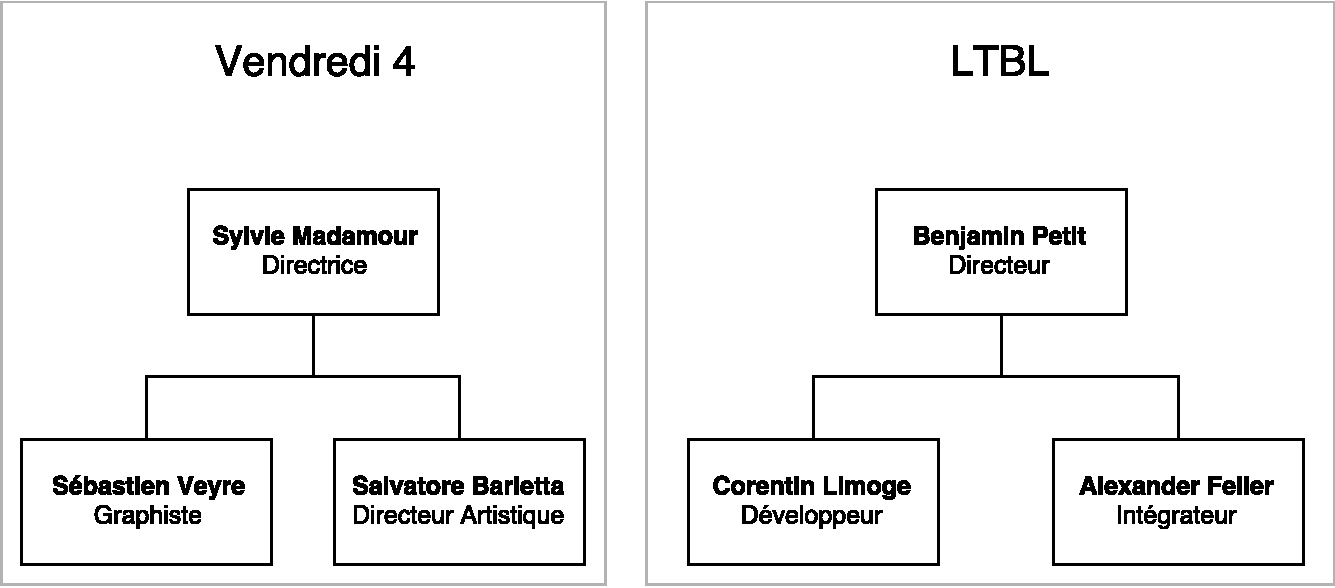
\includegraphics[scale=0.7]{Structure-LTBL.pdf}
    \caption{Structure de LTBL et Vendredi 4}
\end{figure}

Les deux entreprises sont très liées, elles partagent les mêmes locaux et communiquent beaucoup ensemble sur les projets en cours et à venir.

On retrouve alors Benjamin \bsc{Petit}, le gérant, et Corentin \bsc{Limoge} du côté LTBL.
Benjamin s'occupe des conseils et de la gestion de l'entreprise.
Il s'occupe aussi de l'aspect technique des installations par le choix des technologies de pointage et d'affichage.
Corentin est employé par LTBL, mais dispose d'un statut d'auto-entrepreneur, on peut alors le considérer comme un consultant.
Corentin est en charge du développement des applications qui seront exécutées sur les installations.

Du côté Vendredi 4, on retrouve Sylvie \bsc{Madamour}, la directrice, Salvatore \bsc{Barletta}, directeur artistique, et Sébastien \bsc{Veyre}, graphiste.
Sylvie est en charge des contrats, devis et de la communication avec les clients.
Salvatore est directeur artistique chez Vendredi 4, il s'occupe de concevoir et présenter les design des installations aux clients.
Sébastien est graphiste et est en charge de représenter les futures interfaces des installations, mais aussi de travailler sur des rendus en Motion Design\footnote{Une technique d'animation graphique ayant pour but de mettre en valeur le mouvement et l'animation.} Pour donner un premier aperçu de la future application pour les clients et les intégrateurs.

\subsection{Projets}

Les deux entreprises travaillent ensemble pour proposer des services suivants :

\begin{itemize}
    \item Conseils techniques
    \item Conseils en interaction
    \item Design graphique
    \item Développement d'applications interactives
    \item Installations
\end{itemize}

Ainsi, les deux entreprises peuvent suivre la production d'une application interactive de sa conception jusqu'à son installation.

\medskip

Les projets suivis par LTBL sont les suivants :

\paragraph{Dispositifs de présentation interactifs} le plus souvent utilisés dans les salons et showrooms, les dispositifs interactifs permettent une présentation des produits de manière esthétique.
L'objectif de LTBL est donc de concevoir cette installation.
Cela passe par la conception du système physique est des composants requis mais aussi par la conception et le développement de l'interface utilisateur qui doit être réactive et esthétique.
La majorité de ce type de projet est la présentation d'informations sur un produit sur un écran tactile

\paragraph{Vidéo Mapping} Le plus souvent présenté lors d'événements, le vidéo mapping consiste en la projection d'une image déformée sur une structure pouvant être un bâtiment ou une installation spécifique.
Cette image utilise une représentation de la structure pour se déformer et épouser sa forme lors de la projection.
Ce type d'installation permet, au travers de jeux de lumière et d'illusions, de donner vie à la structure ou au bâtiment.
On retrouve ce type d'installation à la fête des Lumières de Lyon par exemple.

\paragraph{Conseils techniques ou en interaction} Fort de son expérience dans le domaine de l'interactivité, LTBL peut aussi donner des conseils en interactivité dans le cadre de projets cités plus haut.

\paragraph{Fête des Lumières} La fête des Lumières est une manifestation Lyonnaise prenant place aux endroits importants de la ville.
Cette fête met en lumière de nombreuses installations lumineuses et interactives.
Chaque année, LTBL peut proposer un projet d'installation en rapport avec un bâtiment de la ville sur lequel s'installer.
Ce projet est alors évalué et est accepté ou non en fonction de la faisabilité, l'esthétique et le coût de l'installation.
La dernière fête des Lumières à laquelle a participé LTBL fut celle de 2015 avec une installation nommée "Lumibus".
Cette installation présentait un Bus muni de panneaux LED réagissant aux accélérations et freinages de celui-ci.
Les années précédentes, LTBL a aussi présenté Hi Striker, une installation reprenant le jeu de foire de la massue où les participants doivent taper le plus fort possible sur un capteur à l'aide d'une massue.
Plus la frappe est forte plus le bâtiment s'illumine.
Cette installation se trouvait au palais de justice.
Plus récemment, LTBL a participé à la fête des Lumières de Hong Kong avec un projet reprenant le même principe, mais en animant un dragon.

\begin{figure}[h]
    \centering
    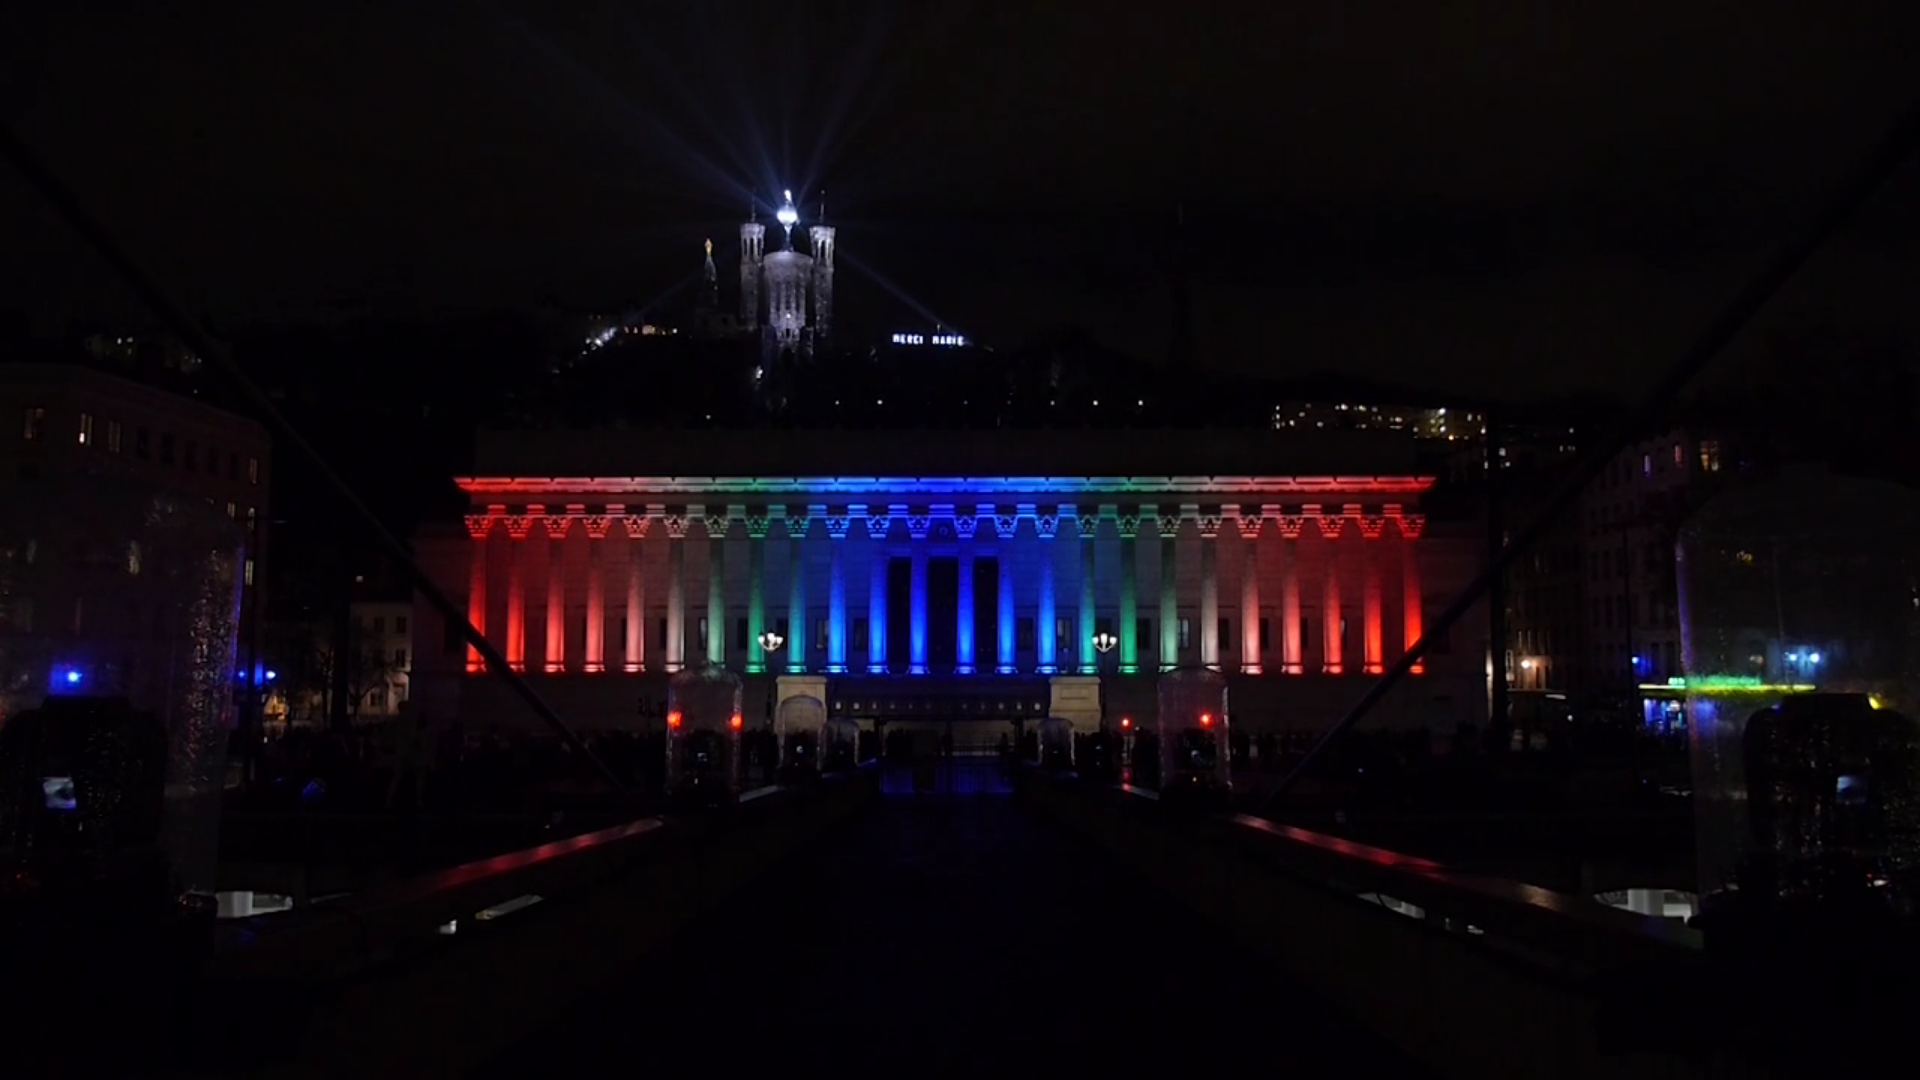
\includegraphics[scale=0.2]{hi-striker.png}
    \caption{L'installation "Hi Striker" à la fête des Lumières de Lyon}
\end{figure}


\begin{figure}[h]
    \centering
    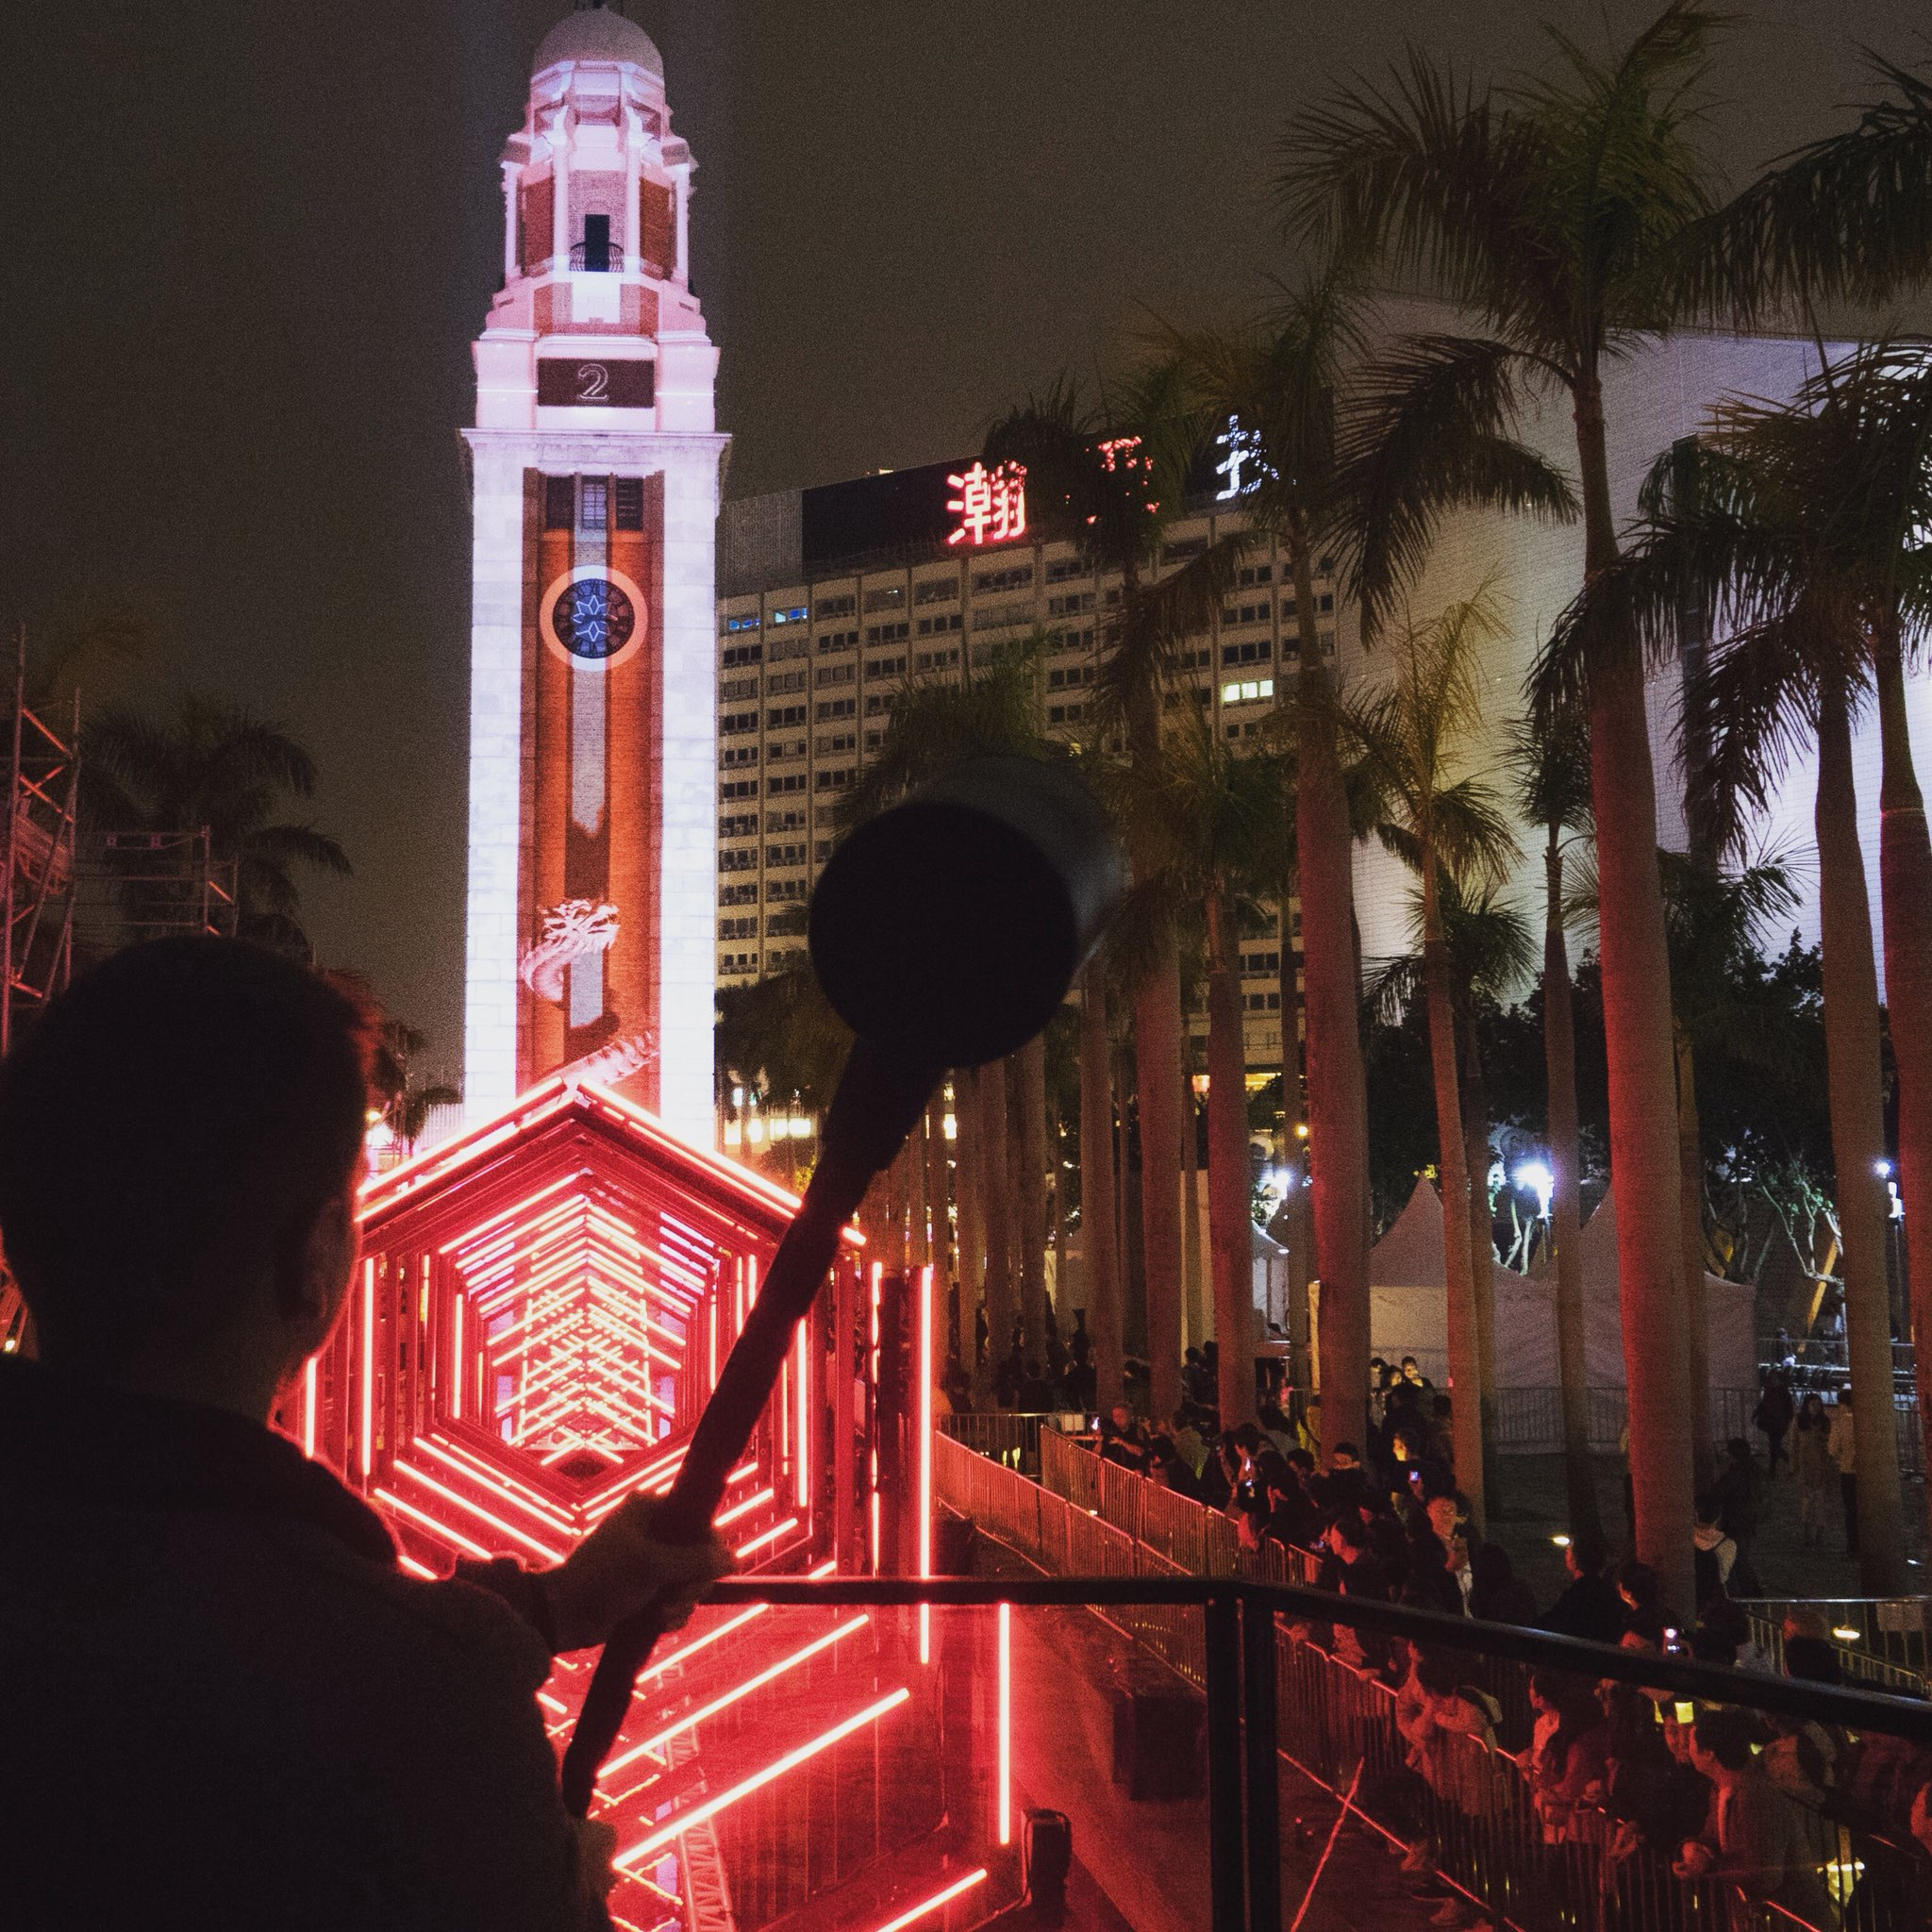
\includegraphics[scale=0.15]{long-striker.jpg}
    \caption{L'installation "Long Striker" à la fête des Lumières de Hong Kong}
\end{figure}

\clearpage

\subsubsection{Clients}

Les clients de LTBL et de Vendredi 4 sont, le plus souvent, de la région Rhône-Alpes, mais peuvent aussi être en région parisienne.
Ces clients sont des PME ou des grands groupes désirant de nouvelles installations interactives pour leurs showrooms.
Au travers de ces installations, ils peuvent montrer leur produit de manière esthétique à leurs clients.
Les showrooms ne sont pas les seuls installations organisées par LTBL, on retrouve aussi des présentations de produits pour les salons ou l'affichage de données pour la productivité.

\medskip

Quelques clients :

\begin{itemize}
    \item Biomérieux
    \item EDF
    \item Michelin
    \item Somfy
    \item Visiativ
    \item Courchevel
    \item Fête des Lumières
    \item Et bien d'autres \ldots
\end{itemize}

\section{Intégration}

Mon intégration dans l'entreprise s'est faite très rapidement.

J'ai commencé par passer l'entretien le 27 novembre qui s'est très bien passé.
J'ai découvert une équipe de 2 personnes sympathiques et ayant des projets intéressants.
On m'a informé sur les objectifs de mon stage.

J'ai intégré l'entreprise le 9 janvier.
J'ai alors découvert ma première mission, le développement d'une application Electron pour afficher les produits de l'entreprise Biomérieux.

La première journée fut une journée de mise en place où j'ai pu accéder aux infrastructures de LTBL.
J'ai eu accès à leur dépôt de code sur BitBucket et les conversations de groupe de LTBL et Vendredi 4 sur Slack.
Enfin, j'ai pu me joindre au Trello mis en place pour le projet que j'ai à faire.

Durant ma première semaine, je me suis familiarisé avec ma première mission et les technologies qui l'entourent comme Electron et les WebComponents.
Je connaissais déjà Electron, une solution de développement d'application native avec des outils Web.
En revanche, je ne connaissais pas les WebComponents, un nouveau standard Web permettant de concevoir des tags HTML personnalisés.
Par contre, j'avais déjà utilisé des frameworks JavaScript avec la même philosophie comme VueJS et Angular;
Avec ces compétences que je possédais déjà et l'expérience de Corentin, j'ai pu apprendre ce nouveau système en une journée.

Le début de ma mission fut assez difficile, car, même si je comprenais les objectifs, aucun cahier des charges n'a formellement été rédigé.
Je me suis donc appuyé sur la vidéo en Motion Design de Sébastien pour en déduire les fonctionnalités à implémenter.
De plus, mon maître de stage étant aux États unis pour le CES de Las Vegas, je ne pouvais pas lui parler sur mes horaires de travail ce qui rend la conception de la solution difficile.

En conclusion, les premières semaines de mon stage se sont très bien passées et je me suis intégré dans cette entreprise plus rapidement que dans les autres stages que j'ai effectués.
C'est sûrement dû à l'ambiance bonne enfant et sympathique des équipes et aussi de l'effectif réduit.

\section{Étonnement}

Durant les premières semaines de mon stage, j'ai eu l'occasion de découvrir cette entreprise et ses particularités par rapport aux autres entreprises que j'ai intégrées.

\paragraph{Ambiance} L'effectif réduit de l'entreprise (2 chez LTBL et 3 chez Vendredi 4) permet de s'intégrer très facilement à l'équipe et de communiquer plus aisément.
Il n'est même plus nécessaire d'utiliser le Slack mis en place pour communiquer sur les projets sur les heures de travail.
De plus, les employés de l'entreprise sont passionnés par leur domaine et cela se sent.
Ils sont très qualifiés et curieux dans la technologie qu'ils maîtrisent et m'ont déjà fait découvrir de nombreuses choses.
Enfin, la curiosité de l'équipe les amènent à découvrir de nouvelles technologies même si cela n'est pas l'objectif premier du projet.
Par exemple, l'entreprise a investi dans une imprimante 3D pour expérimenter cette technologie pouvant être utilisée pour la fabrication de structure ou de boîtier.

\paragraph{Deadlines} J'ai remarqué que LTBL est en charge de courts voir très courts projets qui ne sont pas maintenus sur le long terme.
Ma première mission est un projet de développement d'application sur un unique mois.
En effet, la première présentation du produit s'effectuera le 7 février.
La faible maintenance des projets de LTBL est justifiée par le fait qu'ils contrôlent leurs installations du hardware jusqu'au software par le choix des technologies à utiliser et l'installation chez le client.
Ainsi, une fois que l'installation fonctionne, il n'est plus nécessaire de s'en occuper pour qu'elle fonctionne pendant plusieurs mois voir années.

\paragraph{Locaux \& matériels} Les locaux de LTBL sont assez petit et sont partagés par les deux entreprises.
Ces locaux sont composés de 2 bureaux, une salle principale avec mezzanine et une salle de pause.
Cela suffit pour les équipes, mais la période à laquelle je suis arrivée est une période de livraison pour des projets de tables tactiles.
Ainsi, des écrans tactiles de grande taille ont été livrés pour pouvoir tester en conditions réelles les applications.
De plus, au retour de la fête des Lumières de Hong Kong, beaucoup de matériel comme des barres de LED et des vidéoprojecteurs ont été stockés dans les locaux.

\paragraph{Cahier des charges} Contrairement aux projets à l'EXIA et dans les autres entreprises que j'ai côtoyées, LTBL ne rédige pas de cahier des charges spécifique pour chaque projet.
Les demandes du client sont relayés par les personnes en contact avec celui-ci.
Ainsi, les équipes LTBL mettent plus en avant la communication entre les membres que la lecture et l'écriture de fichiers de cahier des charges.

\section{Missions}

Durant mon entretien, on m'a informé des technologies utilisées par l'entreprise dans les différents projets mis en place.
On retrouve \emph{Open frameworks}, un ensemble de librairies en C++ permettant la création d'applications interactives.
L'entreprise utilise aussi beaucoup \emph{Electron}, un fremework permettant de concevoir des applications natives à l'aide des technologies Web.
Electron est très utilisé dans la création d'interfaces, car les langages web sont conçus dans cette optique.
De plus, Electron disposant du moteur de rendu Web de Chrome, il est possible d'utiliser des technologies récentes comme les WebComponents\footnote{Les WebComponents sont des éléments HTML personnalisés créés par le développeur. Ils disposent de leur propre style et de leur propre logique développée en JavaScript.}.

Mon maître de stage m'a fait part d'un problème qu'il aimerait que je travaille durant mon stage.
Actuellement, les applications sont développées une à une sans reprendre d'élément des anciens projets.
L'objectif est donc de concevoir un framework générique permettant de créer des interfaces plus facilement et en évitant de recréer des éléments déjà créé.

Ce framework nommé "Utopia" n'existe pas encore, mais permettra de produire des interfaces à l'aide de WebComponents génériques.
Après la création de ce framework la création de l'application se résumerait à créer l'interface à l'aide des components génériques, à créer le style de l'application à l'aide d'un CSS spécifique et enfin à créer les éventuels WebComponents manquants.

\subsection{Biomérieux}

Ma première mission fut la création d'une application permettant de présenter les produits de la société Biomérieux dans leurs showrooms.
Après discussion avec mon maître de stage et le graphiste en charge du design de l'application j'ai pu en dégager les fonctionnalités à implémenter.

\medskip

\begin{itemize}
    \item Une application présentant les produits, organisés en thématiques et familles
    \item Chaque produit dispose d'une galerie d'images permettant d'afficher plus d'informations à son sujet
    \item Le client dispose d'un back-office\footnote{Interface secondaire uniquement vue par l'administrateur permettant de gérer les données de l'application.} Permettant de gérer les produits affichés.
    \item Le design doit coller à la charte graphique imposée par Biomérieux et au design créé par le graphiste
    \item L'interface doit être dynamique, animée et esthétique
\end{itemize}

\subsubsection{Technologies}

Pour ce projet, j'ai utilisé \emph{Electron} qui permet de créer des interfaces facilement à l'aide des technologies Web.
Cela permet d'avoir une interface simple à produire tout en ayant les fonctionnalités natives comme le chargement de fichiers depuis le système.

Pour le stockage des données, j'ai opté pour une base de données \emph{SQLite} permettant un stockage dans un fichier sans serveur superflu.
En effet, SQLite est une librairie C mettant à disposition un langage SQL et un stockage de données dans un fichier.
Cette technique est très intéressante dans notre cas, car les données ne seront qu'utilisées par l'application.
De plus, l'application ne nécessite pas de grandes performances et donc pas d'optimisation particulière que peuvent présenter les serveurs SGBDR\footnote{Système de Gestion de Bases de Données relationnelles} comme MariaDB ou PostgreSQL\@.

Enfin, pour gérer ces données j'utilise \emph{Sequelize}, un ORM JavaScript permettant de communiquer avec la base de données.
Cette librairie permet de représenter les données sous forme d'objets JavaScript pour éviter d'écrire les requêtes à la main et ainsi avoir une meilleure intégration des données dans l'environnement JavaScript.

\subsubsection{Structure}

Ce projet fut pour moi l'occasion d'expérimenter mon idée de la structure pour le framework "Utopia".
Pour cette structure, j'ai puisé dans mes connaissances acquises durant ma formation pour concevoir un système en 3 blocs.

\paragraph{Modèle} Le bloc de modèle définissant les données à stocker dans une base de données relationnelle standard.
Pour ce faire, j'utilise la librairie d'ORM \emph{Sequelize} ayant pour avantage d'être compatible avec la majeure partie des bases de données relationnelles actuelles.
Dans cet ORM, on doit définir un modèle, ce modèle sera utilisé pour créer les tables de la base de données.
Le modèle est donc défini dans un unique fichier \texttt{model.js} permettant de centraliser leurs déclarations.

\paragraph{Backoffice} Le back-office est un serveur web exécuté au sein de l'application Electron.
Ce serveur web se base sur le modèle pour créer les formulaires de saisie des données.
Le back-office ne présente aucun code spécifique au modèle de biomérieux, mais met en place une arborescence de formulaires générés en fonction du modèle défini par le développeur.
Cette technique permet de réutiliser ce back-office dans un tout autre contexte.
En effet, il suffit de changer le modèle pour que les formulaires de saisie changent dans le back-office.

\paragraph{Affichage client} L'affichage client représente tout ce qui va être affiché par l'application Electron sur le terminal.
Cet affichage est le seul qui sera vu par les visiteurs du showroom.
Dans l'architecture utilisée, c'est la seule partie spécifique.
Dans cette partie, on utilise les WebComponents pour concevoir l'application.

Parmi ces WebComponents, j'en ai créé des génériques permettant d'effectuer des tâches de base.
Ces WebComponents génériques sont donc :
\begin{itemize}
    \item \texttt{<data-element>} permettant de faire une requête dans la base de données s'actualisant à chaque changement
    \item \texttt{<page-router>} permettant d'afficher ou non une page en fonction de l'URL associée
    \item \texttt{<animation-block>} permettant d'animer des éléments de l'interface en utilisant les transitions CSS
\end{itemize}

\begin{landscape}
    \begin{figure}[h]
        \centering
        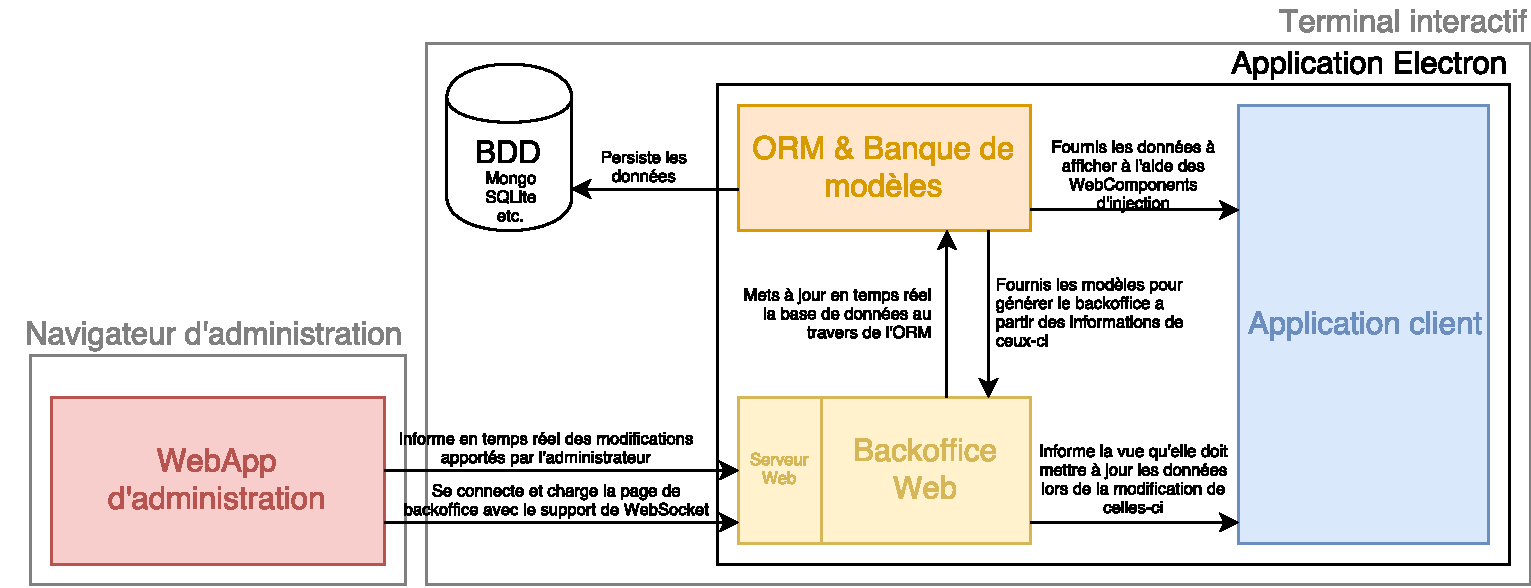
\includegraphics[scale=0.9]{Proposition-utopia.pdf}
        \caption{Structure générale de l'application Biomérieux}
    \end{figure}
\end{landscape}

\clearpage

\subsubsection{Design}

Le design de cette application est fourni par le graphiste de Vendredi 4 et se présente en une suite d'images représentant les différentes pages de l'application.
Ce design présente aussi une vidéo permettant de se représenter les différentes animations de l'application.

\begin{figure}[h]
    \centering
    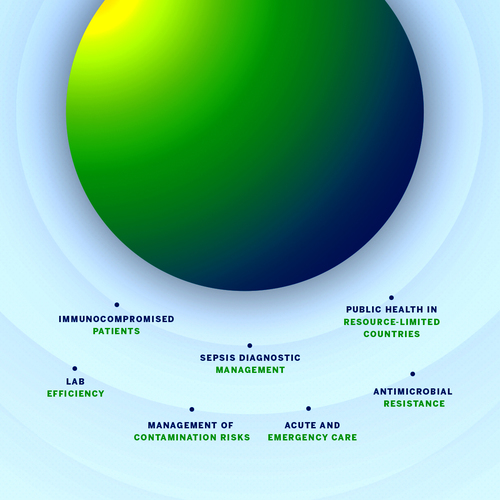
\includegraphics[scale=0.195]{resized-bmx-1-initial.jpg}
    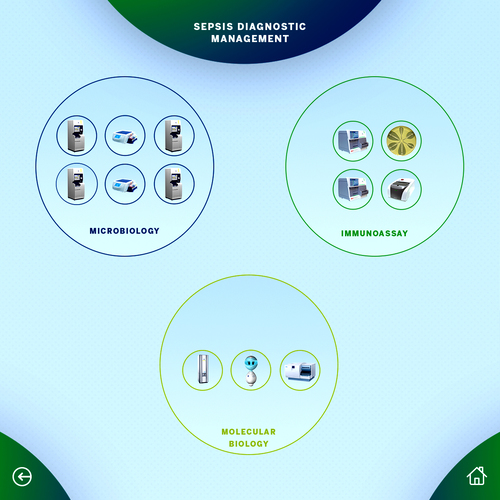
\includegraphics[scale=0.39]{resized-bmx-2-initial.jpg}
    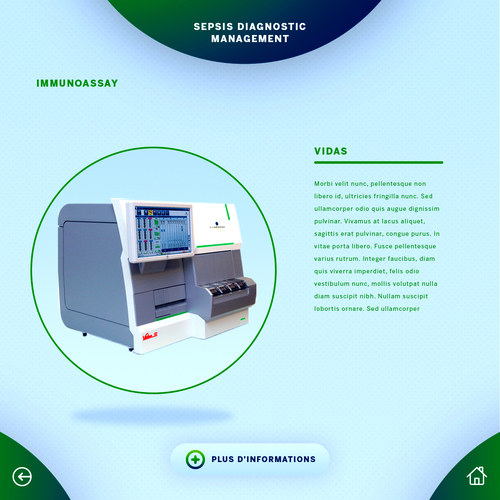
\includegraphics[scale=0.195]{resized-bmx-3-initial.jpg}
    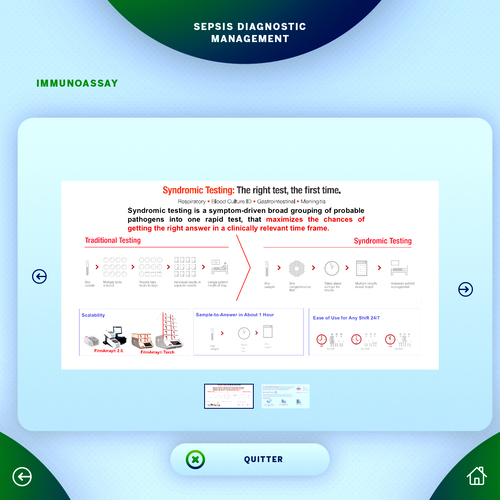
\includegraphics[scale=0.195]{resized-bmx-4-initial.jpg}
    \caption{Design initial de l'application Biomérieux}
\end{figure}

Cependant, ce design a été fait en même temps que le remaniement de la charte graphique de la société.
Il en résulte que ce design ne correspond pas à la nouvelle charte graphique et qu'il fallait de revoir pour qu'il se plie aux nouvelles directives, nouveau logo et nouvelle palette de couleur.

\begin{figure}[h]
    \centering
    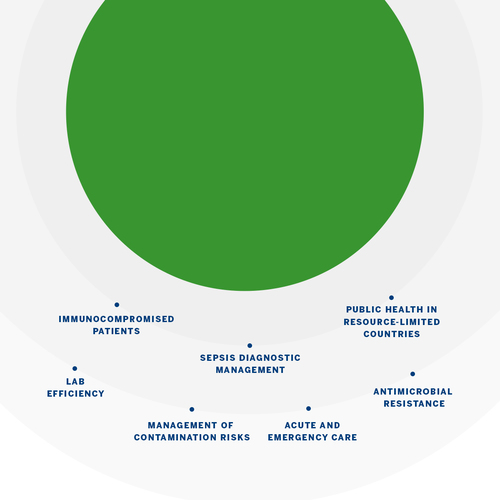
\includegraphics[scale=0.195]{resized-bmx-1-new.jpg}
    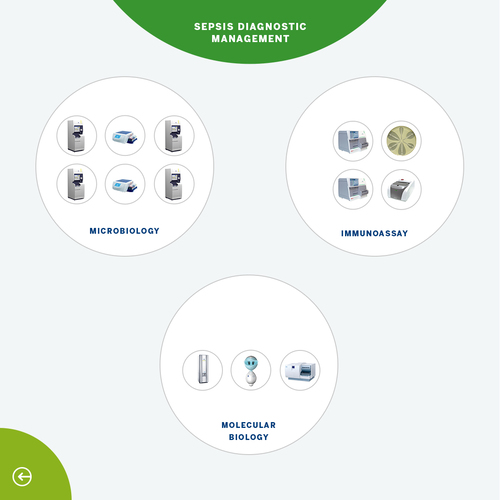
\includegraphics[scale=0.195]{resized-bmx-2-new.jpg}
    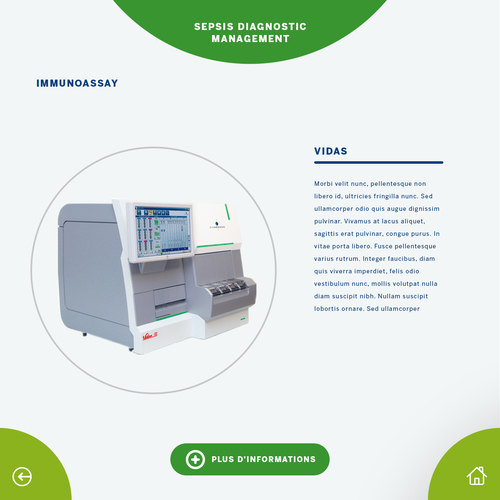
\includegraphics[scale=0.195]{resized-bmx-3-new.jpg}
    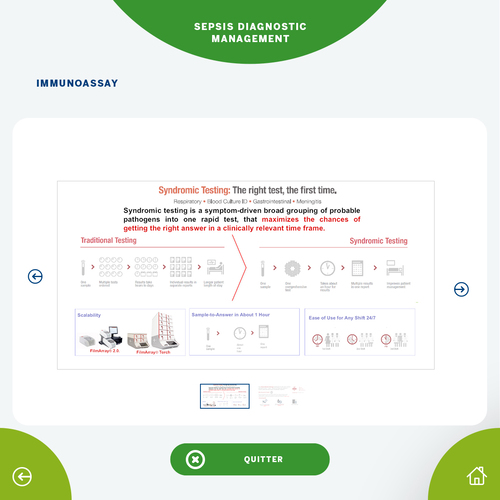
\includegraphics[scale=0.195]{resized-bmx-4-new.jpg}
    \caption{Design renouvelé de l'application Biomérieux}
\end{figure}

\subsubsection{Conclusion}

Ce projet fut une bonne introduction aux techniques des WebComponents et à la manière de travailler des équipes LTBL\@.

Dans ce projet, j'ai opté pour une structure très classique ressemblant à un site Web.
Avec le recul, je me rends compte qu'il y a peut-être une solution plus simple et plus flexible et que la solution que j'ai proposée demande trop de création pour pas grand-chose.
Par exemple, il n'est pas nécessaire de penser les données en amont de l'application, car, dans ce type d'installation, l'apparence finale prévaut sur le contenu.
On peut imaginer un système ou l'on arrange des WebComponents au lieu de générer l'interface sur la base de données.

Ce projet dure depuis 3 semaines et arrive bientôt à son terme avec une première présentation au client le 7 février.

\subsection{Installation au salon de l'entreprise du futur}

Une partie du travaille chez LTBL passe par l'installation des systèmes développés chez le client.
J'ai eu l'occasion de participer à l'installation d'un projet d'écran transparent au salon de l'entreprise du futur.

L'entreprise du futur est un collectif d'entreprise ayant pour objectif d'accompagner ces membres dans la transformation numérique.
À l'occasion du salon de l'entreprise du futur à la cité international, LTBL à aménager 4 écrans transparents permettant de mettre en valeur un produit placé a l'intérieur.
Le produit est alors entouré d'informations sur la société en question.

\begin{figure}[h]
    \centering
    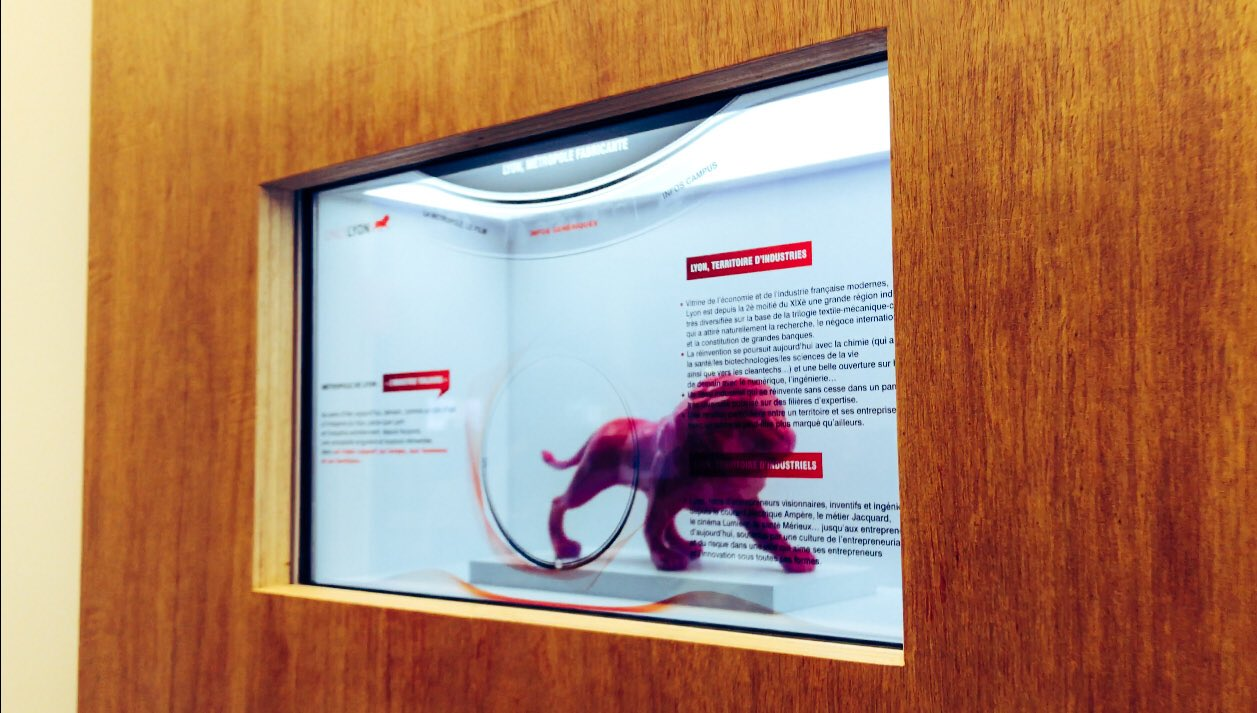
\includegraphics[scale=0.3]{ecran-transparent.jpg}
    \caption{Écran transparent "Only Lyon" au salon de l'entreprise du futur}
\end{figure}

\subsubsection{Technologies}

Pour l'affichage, on utilise des écrans transparents disposant d'une plaque à cristaux liquides permettant d'afficher des informations et d'un compartiment uniformément éclairé en blanc permettant d'y placer un produit.
Sur cet écran s'affichent les informations sur le produit et des vidéos.

Pour afficher toutes ces informations, on utilise un mini ordinateur Asus VivoStick sous Windows 10 avec un site internet affiché en plein écran avec Google Chrome.

Une enceinte USB est disposée au-dessus de l'écran pour diffuser le son des vidéos.

\subsubsection{Conclusion}

Malgré que je n'ai pas travaillé sur ce projet, l'installation fut très intéressante.
Je n'avais jamais fait ce type d'intervention et j'ai appris beaucoup de choses sur les éléments à mettre en place pour éviter tout problème.
Que ce soit par les systèmes empêchant l'utilisateur de sortir de l'application de présentation ou par rapport à l'utilisation futur du projet.

\subsection{Blind Test AccorHotels}

L'objectif de ce projet était de créer une installation permettant de jouer à un Blind Test sur un écran de l'hôtel à l'aide d'un iPad fourni.
Le jeu est simple : Une chanson est jouée sur l'écran et le titre de cette chanson est indiqué.
Le joueur dispose alors de 45 secondes pour trouver l'artiste en question parmi les 4 proposés.
On enchaîne ainsi sur 6 questions qui se terminent sur le résultat du jeu affiché à l'utilisateur.

Le défi sur ce projet fut la deadline.
Pour pouvoir travailler sur des projets plus complexes et importants, mon maître de stage a mobilisé toute l'équipe LTBL composée de Corentin et moi-même pour terminer ce projet dans les plus brefs délais.
Je me suis donc occupé du serveur de jeu quand Corentin s'est occupé de l'affichage sur l'écran et sur l'iPad.

Ce projet fut l'occasion pour moi d'expérimenter le travail d'équipe dans cette entreprise.
Il fallait que je définisse en premier l'interface de communication pour que Corentin puisse l'utiliser pour afficher les données.
Puis, concevoir le système de jeu le plus rapidement possible tout en étant sûr que cela puisse s'adapter au mieux aux exigences présentes et futures du client.

\subsubsection{Technologies}

Les technologies utilisées dans ce projet sont standards et étaient déjà maîtrisées par les membres de l'équipe.
On retrouve alors une application \emph{Electron} pour l'affichage sur l'écran et un serveur NodeJS avec le framework \emph{Express} pour servir les fichiers et gérer le jeu.
Enfin, on utilise \emph{Socket.io} pour les WebSocket apportant de l'interactivité.

\subsection{Structure}

Le Blind Test se compose de 3 éléments.

\paragraph{Le serveur Web} présent dans le processus principal de l'application Electron, il gère tout le jeu du début à la fin.
Il présente un serveur de fichiers permettant l'accès aux fichiers audio, aux fichiers d'image et aux pages Web depuis l'iPad et l'affichage.
Il dispose aussi d'un serveur WebSockets permettant une communication bidirectionnelle entre les clients (iPad et TV) et le serveur.

Ce serveur Web dispose d'un état définissant l'état actuel du jeu.
Cet état est transmis à tous les clients pour qu'ils actualisent leur affichaient lors d'un changement et de la connexion d'un nouveau client.

Le serveur Web construit en parallèle un objet Javascript \texttt{Game} contenant toutes les questions à poser, la question actuellement posée, les réponses des joueurs et le score.
Cet objet \texttt{Game} est transmis à chaque client lors de leur connexion ou lors du changement d'état du jeu.

\paragraph{Les clients (TV et iPad)} Chacun charge une page HTML spécifique possédant un script spécifique.
Ce script va afficher le bon écran en fonction de l'état du jeu envoyé par le serveur et, éventuellement, demander une interaction à l'utilisateur.

Dès qu'un joueur tape sur une réponse, l'iPad envoie à son tour un paquet WebSocket au serveur pour qu'il l'enregistre et change d'état.
Le jeu continue alors jusqu'a ce que toutes les questions de tous les joueurs soient posées.

\begin{figure}[h]
    \centering
    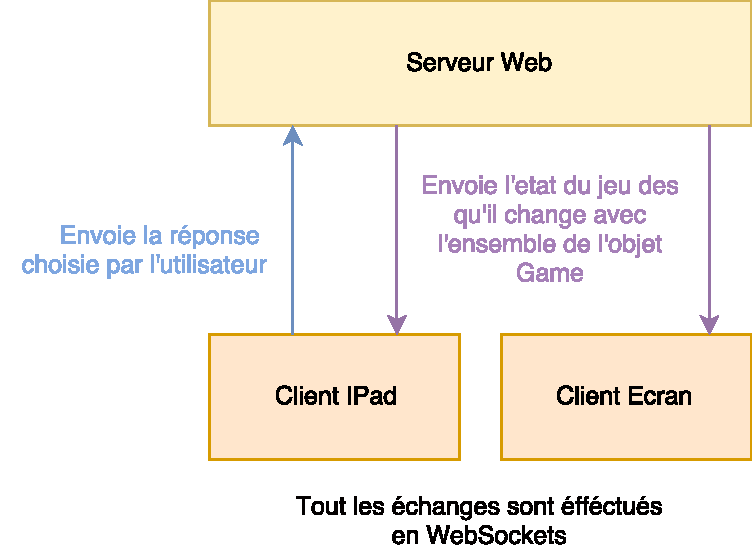
\includegraphics{ah-blindtest.pdf}
    \caption{Structure du jeu Blind Test}
\end{figure}

\subsubsection{Design}

Le design de l'application était fourni avec la demande du client et nous avons juste intégré ce design en extrayant des images clés du fichier Photoshop du designer.

\begin{figure}[h]
    \centering
    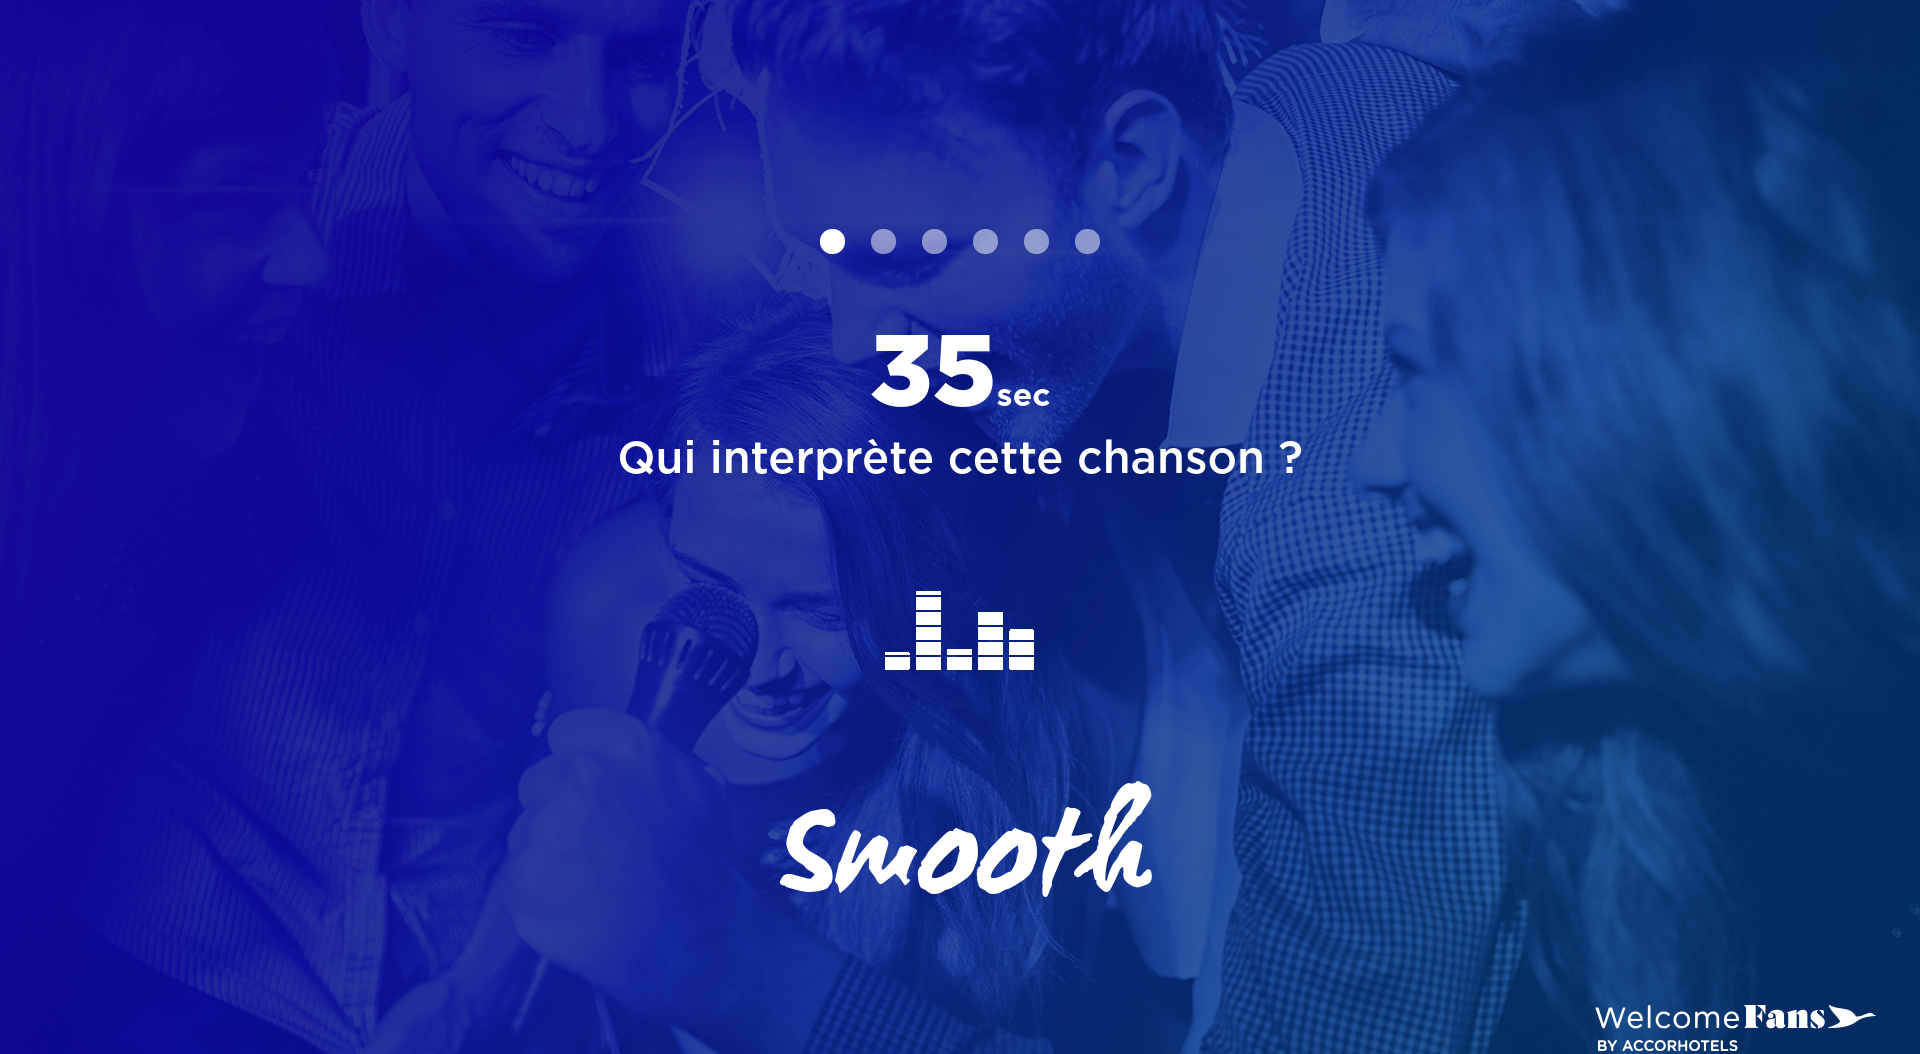
\includegraphics[scale=0.23]{blind-test-tv.png}
    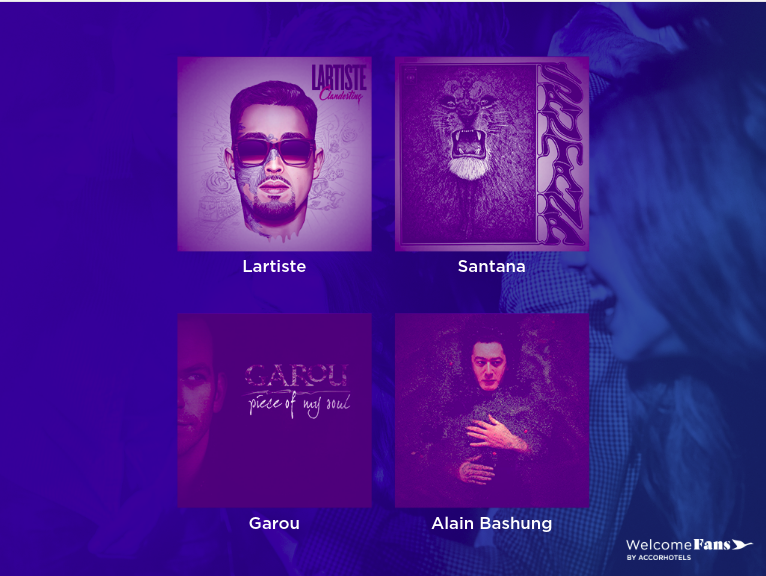
\includegraphics[scale=0.22]{blind-test-ipad.png}
    \caption{Une vue du Blind Test côté TV (à gauche) et côté iPad (à droite)}
\end{figure}

\subsubsection{Conclusion}

Ce projet fut intéressant et intense, car nous l'avons réalisé en seulement 2 jours.
Ce fut une bonne expérience de travail d'équipe et m'a permis de tester un projet à court délai.
L'installation est prévue pour le lundi 29 janvier.

\clearpage

\section{Missions à venir}

Après ces projets, mon maître de stage m'a proposé de travailler sur les projets suivants :

\begin{itemize}
    \item Amélioration d'une table tactile pour Malakoff Médéric : La mise en place d'un back-office
    \item Table tactile de chantier pour Eiffage
    \item Site web de l'entreprise LTBL
    \item Travail sur le framework "Utopia"
    \item Mapping de LED en 3D
\end{itemize}

\section{Conclusion}

Pour conclure, LTBL est une entreprise très différente des autres entreprises que j'ai pu côtoyer.
Chez LTBL, les projets sont rapides et ne demandent pas de grande maintenance.
De plus, la communication entre les membres de l'équipe est au centre des projets et le design un point important de chacune des installations.

J'ai déjà travaillé sur 3 projets chez LTBL, dont 2, du début à la fin.
Le travail effectué m'a permis de remettre en question mes conceptions d'applications pour les adapter au mieux aux demandes du client et aux deadlines imposés.
J'ai déjà appris certaines techniques que je ne connaissais pas comme les WebComponents.

Enfin, j'ai aussi découvert les installations des projets LTBL dans un salon et ce que l'on doit prendre en compte pour garantir une bonne expérience utilisateur.

\section{Bilan}

Ce stage est une très bonne expérience dans un domaine que je ne connais pas et que j'ai rarement côtoyé, celui de l'interactivité.
En effet, les applications que l'on a développées à l'école sont, en grande partie, destinées aux entreprises et le design, l'interactivité et l'attrait pour le grand public n'est pas une priorité.

Aujourd'hui, dans ce stage j'ai l'occasion de travailler avec une équipe qui a des besoins très différents des agences de communications standard.
Chez LTBL, il n'y a pas de serveur de production et de responsive exigé sur les interfaces, mais il y a d'autres contraintes qui sont le design et les animations.

Ce nouveau paradigme me permet de remettre en question mes structures préconçues d'applications pour me faire réfléchir plus en profondeur sur les besoins du client et à mieux prendre en compte les besoins pour le projet.

Malgré que les projets à venir soient aussi sur du Web j'espère pouvoir travailler sur de nouvelles technologies comme le jeu vidéo ou le Mapping Vidéo.

\end{document}
